\chapter{Durchführung}
\label{cha:Durchführung}
In diesem Kapitel wird der verwendete experimentelle Aufbau erklärt, sowie die Durchführung dieses Versuches erläutert. Eine Skizze des verwendeten Versuchaufbaus ist in Abbildung 
\ref{fig:skizze_aufbau} dargestellt.

\begin{figure}
              \centering
              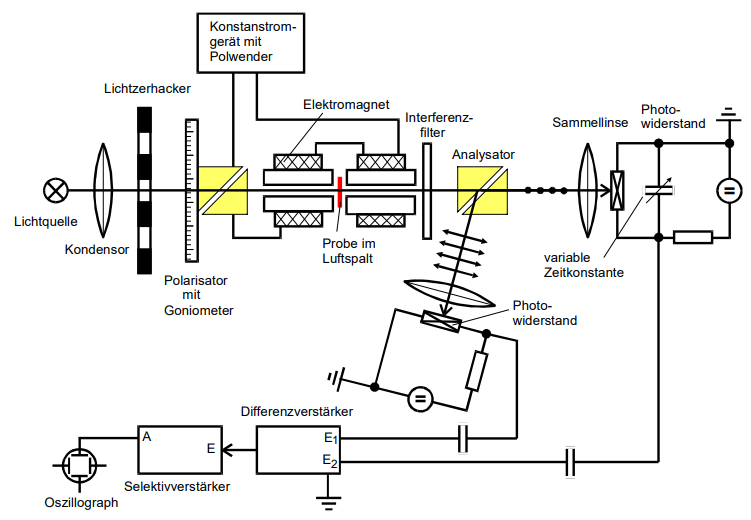
\includegraphics[width = \textwidth]{content/aufbau_skizze.PNG}
              \caption{Skizze des Versuchaufbaus zur Messung des Faraday-Effekts. \cite{v46}}
              \label{fig:skizze_aufbau}
\end{figure}

Die verwendeten Halbleiterproben \ce{GaAs} sind hauptsächlich im Infrarot-Spektrum durchlässig. Daher wird als Strahlungsquelle eine Halogenlampe verwendet, welche ebenfalls 
hauptsächlich in diesem Bereich emittiert. Danach folgt eine Linse, welches das divergente Licht bündelt.
Dann folgt ein Lichtzerhacker. Dieser teilt den Strahlengang des Lichtes in einzelne Bunches auf. Dies ist notwendig,
weil die Photowiderstände durch ihren hohen Innenwiderstand erhebliche Rauschspannungen erzeugen. Das Aufteilen in Bunches ermöglicht dann die Messung über eine Wechsellichtmethode.
Nach dem Zerhacker folgt ein Glan-Thompson-Prisma. Ein solches Prisma nutzt Totalreflexion und Doppelbrechung um lediglich linear-polarisiertes Licht zu propagieren. 
Mithilfe eines Goniometers kann dann der Polarisationswinkel abgelesen 
werden. Darauf folgt dann der Magnet mit einem Luftspalt. Das nun linear-polarisierte Licht propagiert durch den Magneten, in dessen Mitte sich die zu untersuchende Probe befindet. Dort 
tritt dann der Faraday-Effekt auf. Dieser sorgt für eine Rotation in der Polarisation, welche im Kapitel \ref{cha:Theorie} erklärt wurde. Danach folgt ein Interferenzfilter, welcher 
lediglich für bestimmte Wellenlängen transmissiv ist und sonst absorbiert oder reflektiert. Weiter trifft der Strahl dann auf ein zweites Glan-Thompson-Prisma. Diese Prismen haben 
die Eigenschaft das Licht in zwei Strahlengänge mit orthogonaler Polarisation aufzuteilen. Dadurch kann dann ein Zweistrahlenverfahren angewendet werden, welches eine hohe Winkelauflösung 
ermöglicht. Die Intensitäten der beiden Strahlen werden zunächst durch die Photowiderstände gemessen. Die Spannungen werden dann durch einen Differenzversärker und Selektivverstärker 
auf einem Oszilloskop dargestellt. Der Faraday-Winkel kann dann gemessen werden, indem die Differenzspannung minimiert wird. Dabei wird der zugehörigen Winkel am Goniometer abgelesen. 
Dann muss das Magnetfeld umgepolt werden. Dabei wird eine Vorrichtung verwendet, welche hohe Induktionsströme verhindert. Nach der Umpolung wird dann erneut ein Winkel für minimale 
Differenz abgelesen. Da damit zwei mal den Rotationswinkel gemessen wird muss der Winkel über 
\begin{equation}
              \label{eqn:theta}
              \Theta = \frac{1}{2}\left(\Theta_1 - \Theta_2\right)
\end{equation}
berechnet werden.

Damit diese Messung überhaupt funktioniert muss die Messvorrichtung vorher optimal justiert werden. 

Nach der Optimierung des Aufbaus kann die Messung begonnen werden. Zu Beginn muss das maximale Magnetfeld, von welchem der Faraday-Effekt abhänt, bestimmt werden. Dazu wird eine 
Hall-Sonde verwendet. Diese wird in den Magneten eingeführt. Dabei wird immer die Tiefe und die Feldstärke aufgenommen. Besonders interessant ist dabei die Feldstärke im Zentrum
wo die Probe plaziert werden soll. Nachdem das Feld untersucht worden ist, kann eine der drei möglichen \ce{GaAs} Proben in dem Magneten plaziert werden. Für neun verschiedene 
Interferenzfilter/Wellenlängen wird dann die Faraday-Rotaion aufgenommen. Diese Messung wird dann für die zwei weiteren 
Proben wiederholt.   